\section{From completion to construction}
\label{sec:construction}

A completed color group earns little until it is developed. The 63 trade-completed groups let us ask what happened at the first chance to build. All 63 owners reach an actual management window. First-window construction follows for 16 of 17 groups completed by Sol, 17 of 18 by Gemini, 7 of 15 by Opus and 3 of 13 by Grok (Figure~\ref{fig:development}, left).

\begin{figure}[htbp]
\centering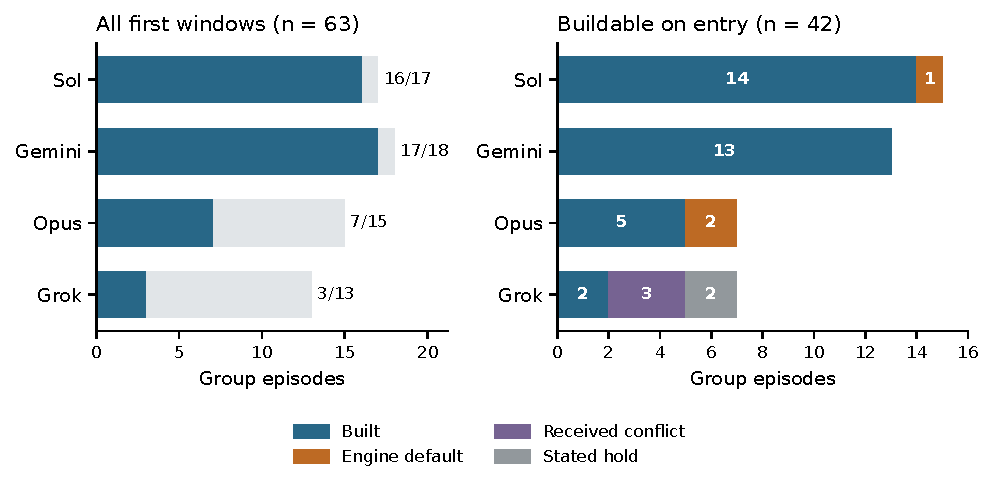
\includegraphics[width=\linewidth]{development.pdf}
\caption{First management window after trade completion. Left, all 63 trade-completed groups. Right, the 42 groups buildable when the window opened, by how the window was resolved. ``Engine default'' is an \End{} applied by the engine after failed attempts; ``received conflict'' is a received \End{} call whose assistant content names another action. Counts carry each configuration's response condition (Table~\ref{tab:conditions}).}
\label{fig:development}
\end{figure}

The twenty unbuilt groups have four different explanations. Nine were never buildable on any menu during the window, all owned by Opus or Grok; the ledger does not record why, and earlier play, cash and jail can each contribute. Four ended in engine defaults, three of them Opus defaults after refusal recovery. Four ended with a received \End{} call whose assistant content asked for something else, all Grok. Only three ended in a valid \End{} with no detected conflict. Restricting to the 42 groups buildable on entry gives 34 built and eight unbuilt: three defaults, three conflicts and two stated holds. Reading all twenty, or all eight, as a decision to keep cash would combine incompatible records.

\subsection{Most \End{} records are not verified holds}

\begin{table}[htbp]
\centering\small
\begin{tabularx}{\linewidth}{lRRRRR}\toprule
Configuration & Menus listing construction & \End{} applied & Engine default & Name conflict & No detected conflict\\\midrule
Sol & 399 & 236 & 4 & 0 & 232 \\
Gemini & 330 & 144 & 1 & 0 & 143 \\
Opus & 223 & 104 & 61 & 0 & 43 \\
Grok & 273 & 179 & 0 & 24 & 155 \\
\midrule Total & 1,225 & 663 & 66 & 24 & 573\\\bottomrule
\end{tabularx}
\caption{Every applied \End{} on a management menu that lists construction. ``No detected conflict'' includes empty or unparseable content and is not a count of verified reserve decisions. Sol and Gemini's assistant content is empty throughout, and 42 of Opus's 43 non-default \End{} records use action-only recovery, so the last two columns cannot be compared as error or intention rates. A listed tool does not mean that any particular allocation was affordable.}
\label{tab:end}
\end{table}

Across the cohort, 1,225 management menus list the construction tool and 663 end with an applied \End{} (Table~\ref{tab:end}). Sixty-six of these are engine defaults and 24 are Grok calls that conflict with named content. The remaining 573 have no detected conflict, which is weaker than saying they are deliberate holds: they include empty content and cases where nothing affordable was worth building. For Opus, 61 of 104 \End{} records are engine defaults.

\subsection{The requested builds were executable}

The defaults are informative because the failed attempts usually say what the agent wanted. The 66 default decisions contain 132 attempts. Seventy attempts hold a well-formed construction target, and every one is invalid as written, usually because a count-valued request breaks even building at an intermediate step. Splitting each request into single purchases and reordering them, with no extra cash, stock or turns, executes 63 of the 70 targets; the other seven cost more than the player's cash. One further target is malformed and 61 attempts contain no parseable target. At the decision level, 63 of 66 defaults contain a reachable requested target: 61 Opus decisions, one Sol and one Gemini. Every one of the 61 defaulted Opus purchase multisets executes after reordering.

The Opus defaults share one path. In 60 of them, the provider refuses the first attempt, the action-only retry submits an invalid build plan, and the exhausted response policy applies \End{}. In the remaining case (G2 d129) the invalid plan comes before the refusal. The other configurations receive a corrective message after an invalid plan and usually recover (Table~\ref{tab:recovery}). After an uneven-building rejection, Sol applies the same purchase multiset in 20 of 29 decisions, Gemini in 6 of 19 and Grok in 5 of 5. Opus does so in 0 of 61, because no retry remains. A different legal build counts as recovering a valid action but not the requested allocation: in G2 d243 Sol's seven-house target could have executed leaving \$208, while the retry and next decision buy six houses and leave \$358.

\begin{table}[htbp]
\centering\small
\begin{tabularx}{\linewidth}{lRRRRR}\toprule
Configuration & Uneven-build rejections & Some build applied & Same multiset & Changed multiset & Default\\\midrule
Sol & 29 & 25 & 20 & 5 & 4 \\
Gemini & 19 & 18 & 6 & 12 & 1 \\
Opus & 61 & 0 & 0 & 0 & 61 \\
Grok & 5 & 5 & 5 & 0 & 0 \\
\bottomrule\end{tabularx}
\caption{Decisions with an uneven-building rejection, followed to resolution within the same decision. The Opus rows follow refusal recovery, which has already used the retry.}
\label{tab:recovery}
\end{table}

Defaults are concentrated, with 55 of 66 in G5 and G13, so the Opus cases describe a few games and repeated targets more than a general rate. In those windows Opus still asked for development it could afford, and the game recorded none.

Valid holds also occur. At G3 d176, under action-only recovery, Opus ends with \$204 and states a preference for reserves over a legal \$150 house, so the refusal condition alone does not make an \End{} engine-authored. At G1 d426 Grok ends with \$488 when another Atlantic house would have cut its liquidation capacity by the \$75 purchase-to-resale loss. These records show stated reserve preferences, not correct ones.

For an economic agent, a sound allocation that cannot be expressed in the interface's action language earns nothing. In this cohort the gap between requested and executed development is a property of the interface (count-valued plans checked entry by entry) together with the retry policy, and it falls almost entirely on one configured system. Comparing construction counts across configurations as a measure of willingness to invest would mistake that interface property for a preference.

\FloatBarrier
